\chapter[System Design]{System Design}

\section{System Design}
% general overview of the system, how every part is integrated, vue app, backend, db, docker etc
In the previous chapter the requirements of the project were illustrated. From these an initial high level overview of the system can be generated as depicted in \autoref{fig:usecases}.


\begin{figure}[H]
    \begin{center}
    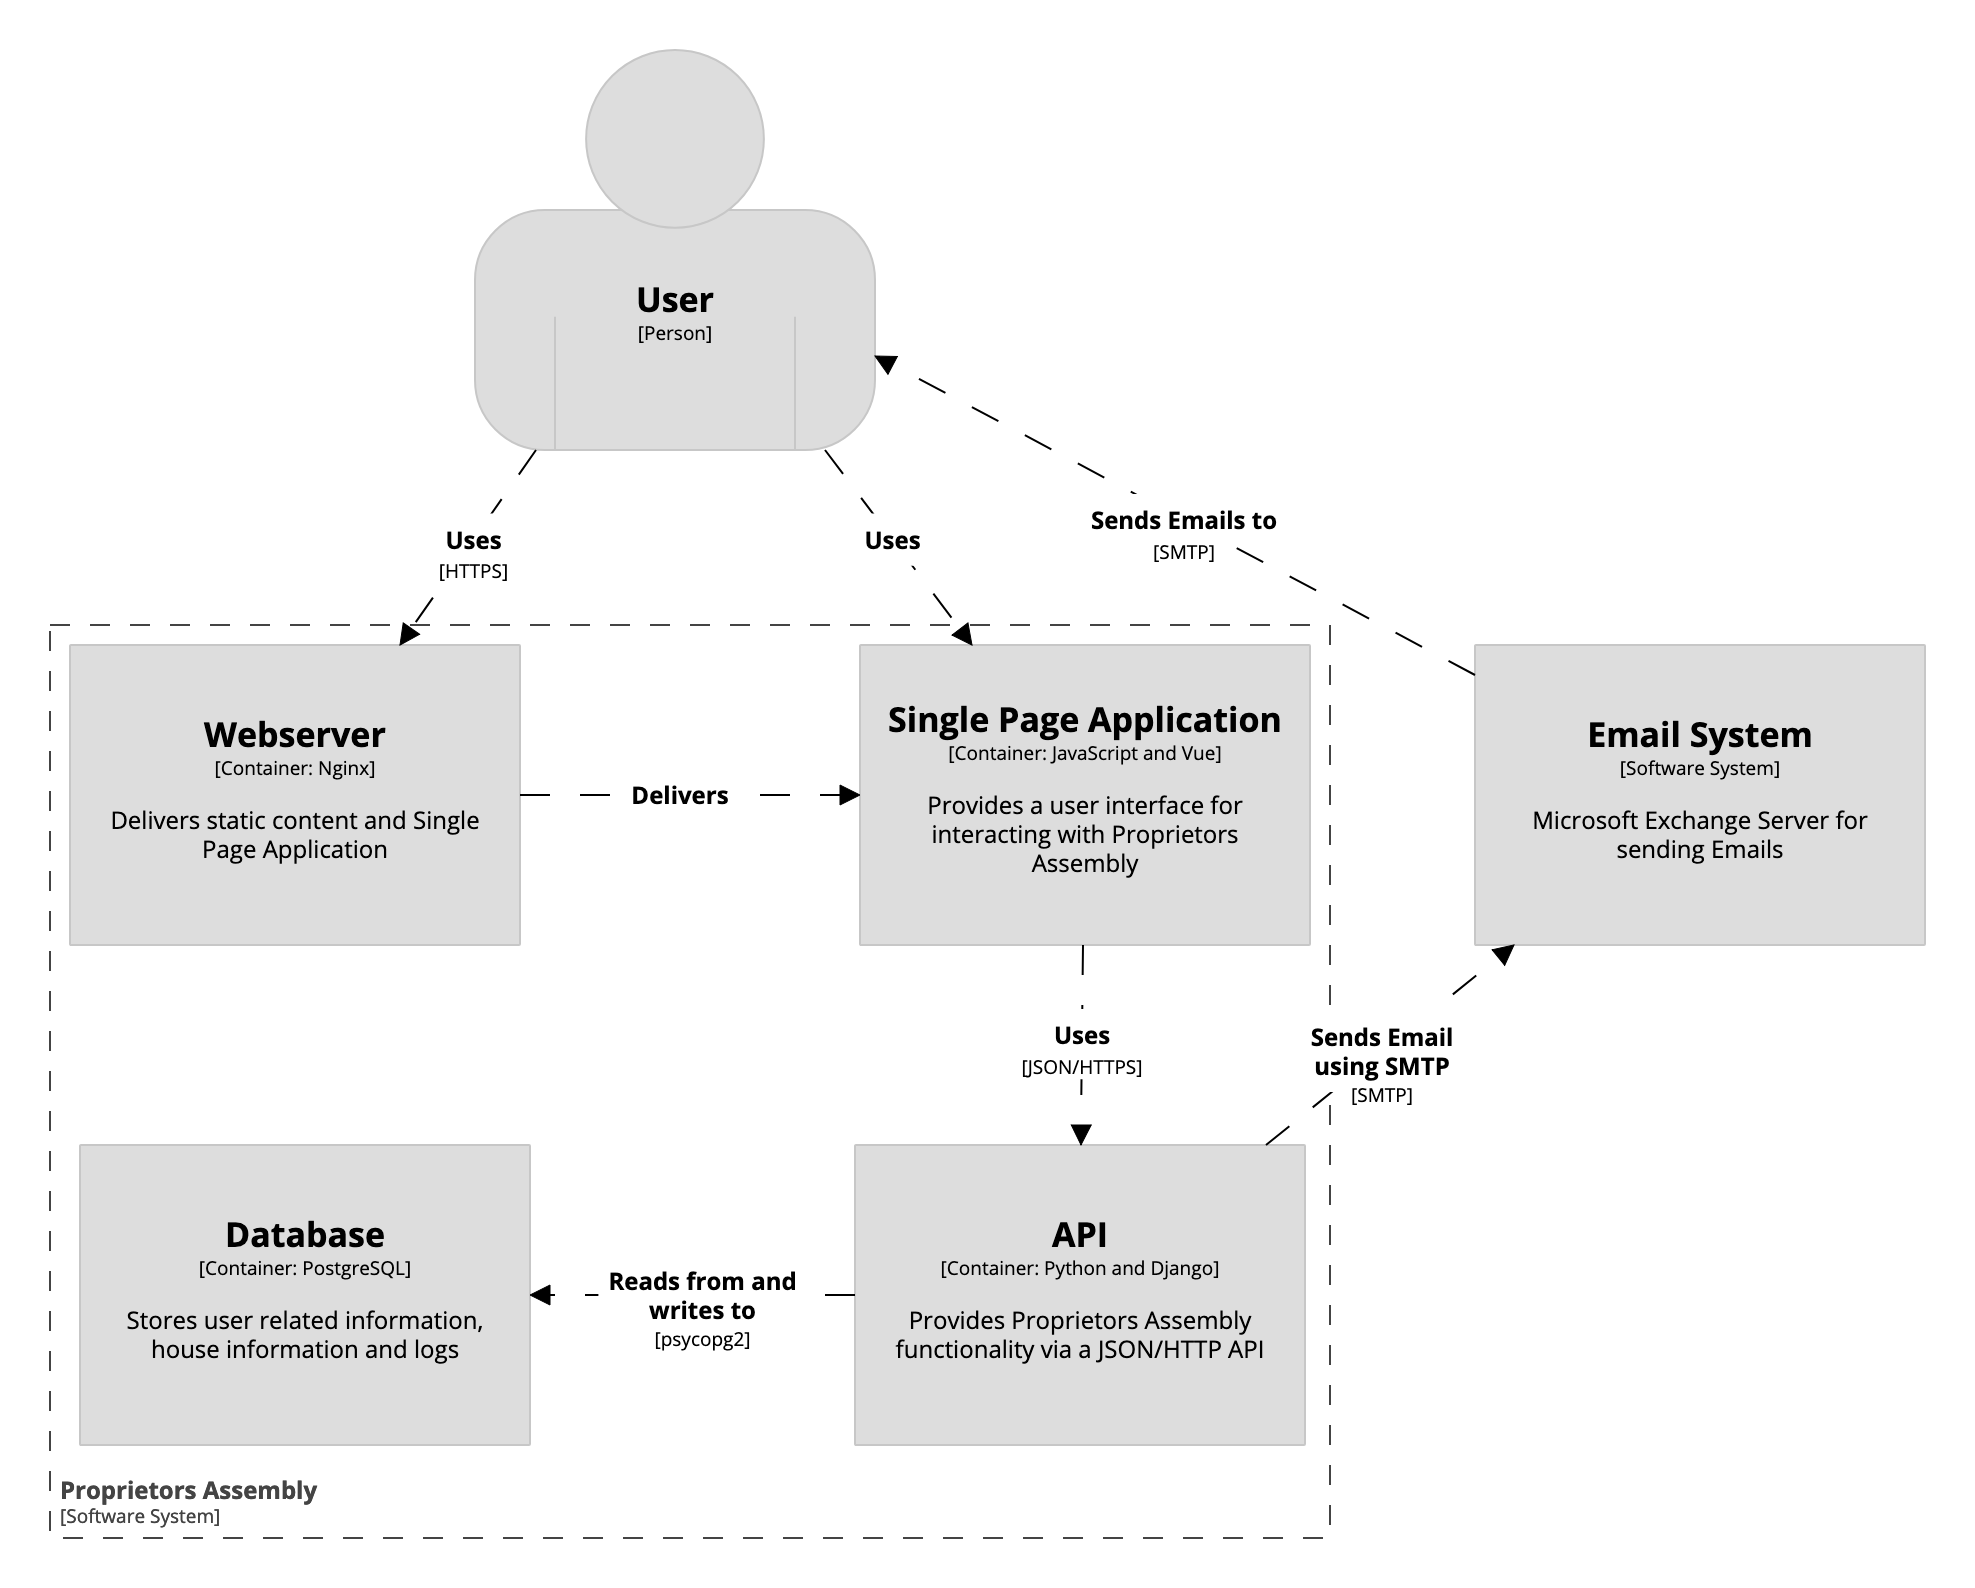
\includegraphics[height=5in]{container_diagram}
    \end{center}
    \caption{System Design}
    \label{fig:usecases}
\end{figure}

In its basic structure, Proprietors Assembly as a software system consists of an NGINX webserver, a Vue \acrlong{spa}, a Django API and a PostgreSQL database. When a user visits the domain \url{https://hausversammlung.at}, the webserver will serve the static frontend which communicates with the API. Depending on the use-case, the API will retrieve data from or add to the Database. An additional third-party Exchange server is used to send emails regarding authentication and house details. The diagram intentioanlly omitts certain parts of the system for brevity. One of these is a reverse-proxy service which is the first point of contact from a user's viewpoint. A reverse proxy in this case routes between containers which are hosted on the same machine, accessible through unique ports. This topic is discussed in depth in \autoref{ch:deployment}.

\section{User Interface Design}
% Defining how to framework should look like, dashboard-like look, what pages have to be created in order to fullfill requirements. Maybe additional wireframes
The UI design of the frontend is strongly dependant on the required functionality. This section aims to translate functional requirements into identifiable elements with no regards to CSS or usability at this point. This makes it possible to detect elements that are used in multiple places and clearly shows the base structure of the frontend. Furthermore, as Vue uses a component-based approach, the identified elements can directly be translated into reusable Vue components.

\subsection{Login Page}
The Login / Register page handles user authentication. A user is required to log into an existing account or create a new one before they can use the system. Traditionally, this is done with a plain HTML-Form. It is sensible to create separate forms for login and register and let the user decide which form to use depending on their needs. \newline

Identified Elements: HTML forms for login and register

\subsection{Home}
On the home site various data sources are composed into a consolidated view - a dashboard. It shows the most recent forum items, polls and noticeboard entries in addition to the current number of issues, house parties and squaremeters. A user should be able to switch between a list of houses they are associated with. A navigation bar should contain links to all subpages: Home [sic], Noticeboard, Polls, Forum, Issue Management and the Profile. \newline

Identified Elements: Noticeboard Item, Poll Item, Forum Item, House Switcher, Navigation Bar

\subsection{Noticeboard}
The Noticeboard page contains a list of all noticeboard entries associated with a house. An input field should let the user search for a specific item. A navigation bar as described for the previous page should allow for page changes. Lastly, a button that links to a page where Noticeboard entries can be created should exist. A Noticeboard item needs to have a title and a message which are entered with a form. \newline

Identified Elements: Noticeboard Item List, Noticeboard Item, Search Bar, Navigation Bar, Create Button, Create Noticeboard Entry Form

\subsection{Polls}
This site contains a list of poll items associated with a house, a way of searching / filtering these and a navigation bar. Creating a poll happens by initially clicking a create button. To create a poll, a title and at least two options have to be provided by the user.

Identified Items: Poll Item List, Poll Item, Search Bar, Navigation Bar, Create Button, Create Poll

\subsection{Forum}
The Forum page shows users a list of all thread items of a house. The items are searchable and a new thread can be created by clicking a button. On the create site a thread can be created which has a title, category and content. Additionally, a navigation bar links to the other pages.

Identified Items: Thread Item List, Thread Item, Search Bar, Navigation Bar, Create Button, Create Thread Form

\subsection{Issue Management}
Similar to the other pages, the issue management page has a navigation bar, a search bar and a button which links to the respective create-site. It shows a list of all house-related issues which. An issue has a reference, date, type, location, title and status.

Identified Items: Issue Item List, Issue Item, Search Bar, Navigation Bar, Create Button, Create Issue Form

\subsection{Profile Page}
On the profile page the user is able to make basic changes to their account such as changing their name. Additionally, they can switch languages or house and invite additional users to their currently selected house. \newline

Identified Elements: Language Switcher, Invite Form, House Switcher

\subsection{Add House Page}
Users need a way of creating a new house or adding an existing house to their account by using an invitation link. To create a new house a form must be provided which takes the address, total squaremeters and role of the user as input variables. An invitation can be accepted by providing an invitation id and the intended role of the user. After creating or accepting an invitation users are given the possibility to invite additional users to their newly added house. \newline

Identified Elements: Create House Form, Accept Invite Form, Invite Form

\section{Summary}
Some Elements are very distinct and are only used once whereas others are used across multiple pages. One element that stands out and is used in almost every single page is the Navigation Bar. It would be very sensible to not only create a reusable component of this element but to also include it in some kind of base-layout. Some other widely used elements are: a Search Bar and a Create Button. Other elements which might not be used very often but reused nevertheless are the Language Switcher and House Switcher. The various forms, lists and items mentioned previously are used only once most of the time, however, it still makes sense to create reusable Vue components for these to make site composition easier.

\begin{figure}[H]
    \begin{center}
    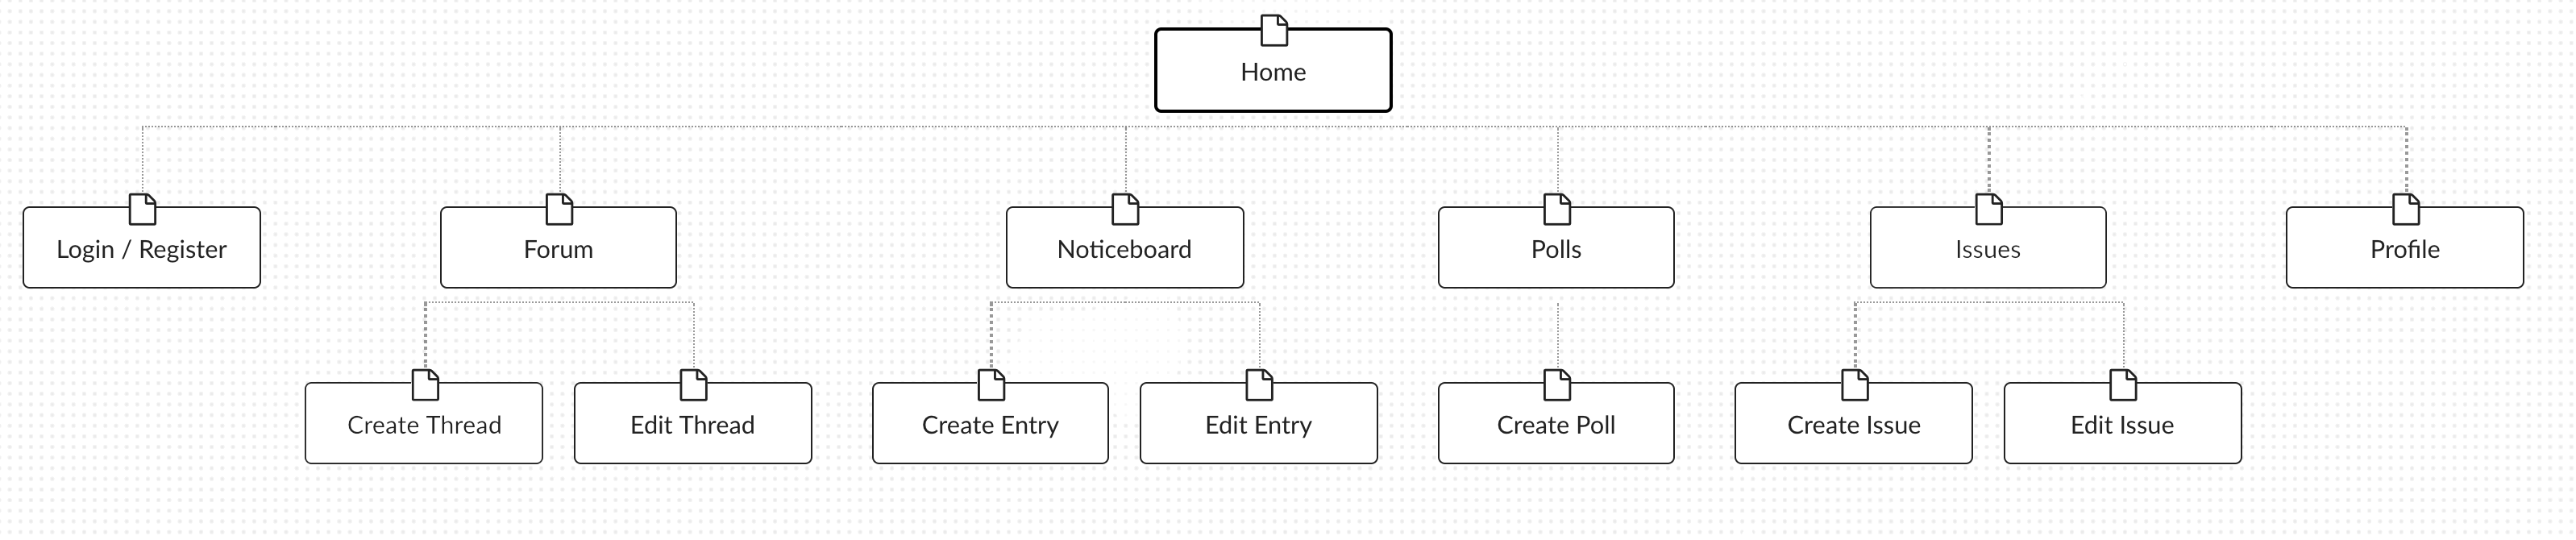
\includegraphics[height=1.4in]{sitemap}
    \end{center}
    \caption{System Design}
    \label{fig:usecases}
\end{figure}

